\begin{figure}
\centering

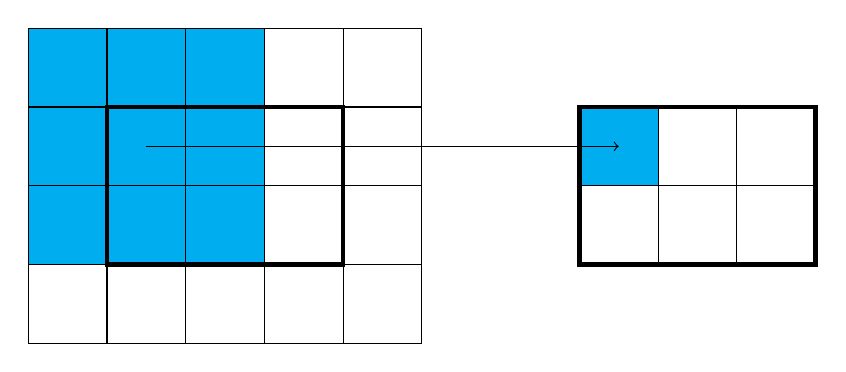
\begin{tikzpicture}
%  , fill=black!20!white
\draw [draw=black, fill=cyan] (0,1) rectangle (3,4);
\draw [draw=black, ultra thick] (1,1) rectangle (4,3);
\draw [draw=black] (0,0) grid  (5,4);

\draw [draw=black, fill=cyan] (7,2) rectangle (8,3);
\draw [draw=black, ultra thick] (7,1) rectangle (10,3);
\draw [draw=black] (7,1) grid  (10,3);

% ,very thick
\draw [->] (1.5, 2.5) -- (7.5, 2.5) ;

\end{tikzpicture}

\caption{Applying a $3 \times 3$ filter to a layer of size $4 \times 5 \times 1$. Note how the $3 \times 3$ region is reduced to a single unit and how the size of the activation map is decreased after the operation.}
\label{fig:filter}
\end{figure}
